\documentclass[18pt]{beamer}
\usepackage[utf8]{inputenc} % for the umlauts
\usepackage{subfigure}

\beamertemplatenavigationsymbolsempty
%% SLIDE FORMAT

% use 'beamerthemekit' for standard 4:3 ratio
% for widescreen slides (16:9), use 'beamerthemekitwide'

\usepackage{templates/beamerthemekit}
% \usepackage{templates/beamerthemekitwide}

\setcounter{tocdepth}{1}

%% TITLE PICTURE

% if a custom picture is to be used on the title page, copy it into the 'logos'
% directory, in the line below, replace 'mypicture' with the 
% filename (without extension) and uncomment the following line
% (picture proportions: 63 : 20 for standard, 169 : 40 for wide
% *.eps format if you use latex+dvips+ps2pdf, 
% *.jpg/*.png/*.pdf if you use pdflatex)

%\titleimage{mypicture}

%% TikZ INTEGRATION

% use these packages for PCM symbols and UML classes
% \usepackage{templates/tikzkit}
% \usepackage{templates/tikzuml}

% the presentation starts here

\usepackage{mathabx}
\usepackage{picture}
\usepackage[absolute,overlay]{textpos}
%\usepackage[texcoord,grid,gridunit=mm,gridcolor=red, subgridcolor=green]{eso-pic}
\setbeamercovered{invisible}
\setbeamertemplate{caption}{\raggedright\insertcaption\par}

\title[SWT1]{Softwaretechnik 1 - 3. Tutorium}
\subtitle{Tutorium 03}
\author{Felix Bachmann}
\date{12.06.2017}

\institute{KIT - Institut für Programmstrukturen und Datenorganisation (IPD)}

% Bibliography

\usepackage[citestyle=authoryear,bibstyle=numeric,hyperref,backend=biber]{biblatex}
\addbibresource{templates/example.bib}
\bibhang1em

\begin{document}

% change the following line to "ngerman" for German style date and logos
\selectlanguage{ngerman}

%title page
\begin{frame}
\titlepage
\end{frame}

\begin{frame}
\tableofcontents
\end{frame}


\section{Orga}
	\subsection{Feedback 2. Übungsblatt}
	\begin{frame}
		\frametitle{2. Übungsblatt Statistik}
		%TODO statistics 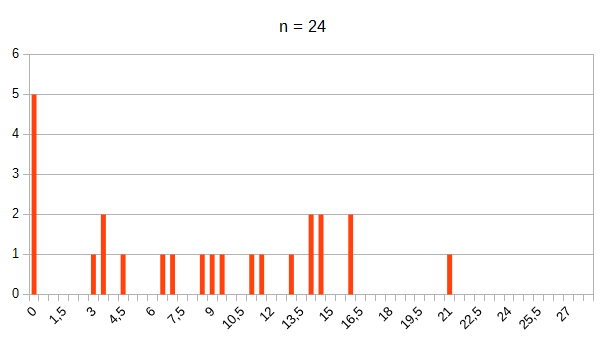
\includegraphics[scale=0.7]{./pics/tut2/statistics-ub2.png}
		%TODO \linebreak \centering $\diameter$ 8,35 bzw. 11,79 von 25 (28)
	\end{frame}

	
	\subsection{2. Übungsblatt - Fehler (Allgemein)}
	\begin{frame}
		\frametitle{Häufige Fehler}
		\begin{block}{Allgemein}
			\begin{itemize}
				\item 			%TODO common faults
			\end{itemize}
		\end{block}
	\end{frame}
	
	\subsection{3. Übungsblatt - Fehler}
	\begin{frame}
		\frametitle{Häufige Fehler}
		\begin{block}{Aufgabe 1 (Plug-In-Architektur): $\diameter$  von 4 (+ 1)} %TODO avg
			\begin{itemize}
				\item %TODO
			\end{itemize}
		\end{block}
	\end{frame}

	\begin{frame}
		\frametitle{Häufige Fehler}
		\begin{block}{Aufgabe 2 (Plug-In): $\diameter$ von 4} %TODO avg
			\begin{itemize}
				\item 	%TODO
			\end{itemize}
		\end{block}
	\end{frame}

	\begin{frame}
		\frametitle{Häufige Fehler}
		\begin{block}{Aufgabe 3 (iMage-Bundle): $\diameter$  von 2} %TODO avg
			\begin{itemize}
				\item 	%TODO
			\end{itemize}
		\end{block}
	\end{frame}

	\begin{frame}
		\frametitle{Häufige Fehler}
		\begin{block}{Aufgabe 4 (Aktivitätsdiagramme (Geometrify)): $\diameter$ von 10} %TODO avg
			\begin{itemize}
				\item 	%TODO
			\end{itemize}
		\end{block}
	\end{frame}

	\begin{frame}
		\frametitle{Häufige Fehler}
		\begin{block}{Aufgabe 5 (Sequenzdiagramm (main-Methode)): $\diameter$ von 5} %TODO avg
			\begin{itemize}
				\item %TODO
			\end{itemize}
		\end{block}
	\end{frame}

	\begin{frame}
		\frametitle{Häufige Fehler}
		\begin{block}{Aufgabe 6 (Substitutionsprinzip): $\diameter$ von 3} %TODO avg
			\begin{itemize}
				\item 	%TODO
			\end{itemize}
		\end{block}
	\end{frame}



\section{Tipps}
	\subsection{Tipps}
	\begin{frame}
		\frametitle{Tipps - 4. Übungsblatt}
			\begin{exampleblock}{Aufgabe}
				\begin{itemize}
					\item 	%TODO
				\end{itemize}
			\end{exampleblock}
			\pause
			\begin{exampleblock}{Aufgabe}
				\begin{itemize}
					\item %TODO
				\end{itemize}
			\end{exampleblock}
	\end{frame}

	\begin{frame}
		\frametitle{Tipps - 4. Übungsblatt}
			\begin{exampleblock}{Aufgabe}
				\begin{itemize}
					\item %TODO
				\end{itemize}
			\end{exampleblock}
			\pause
			\begin{exampleblock}{Aufgabe}
				\begin{itemize}
					\item 	%TODO
				\end{itemize}
			\end{exampleblock}
	\end{frame}
	
	\subsection{Abgabe}
	\begin{frame}
		\frametitle{Denkt dran!}
		\begin{alertblock}{Abgabe}
			\begin{itemize}
				\item Deadline am 21.6 um 12:00 %TODO check when released
				%TODO more to remember?
			\end{itemize}
		\end{alertblock}
	\end{frame}
		
	\begin{frame}
		\frametitle{Bis dann! (dann  := 26.06.17)}
		\centering
		%TODO choose comic 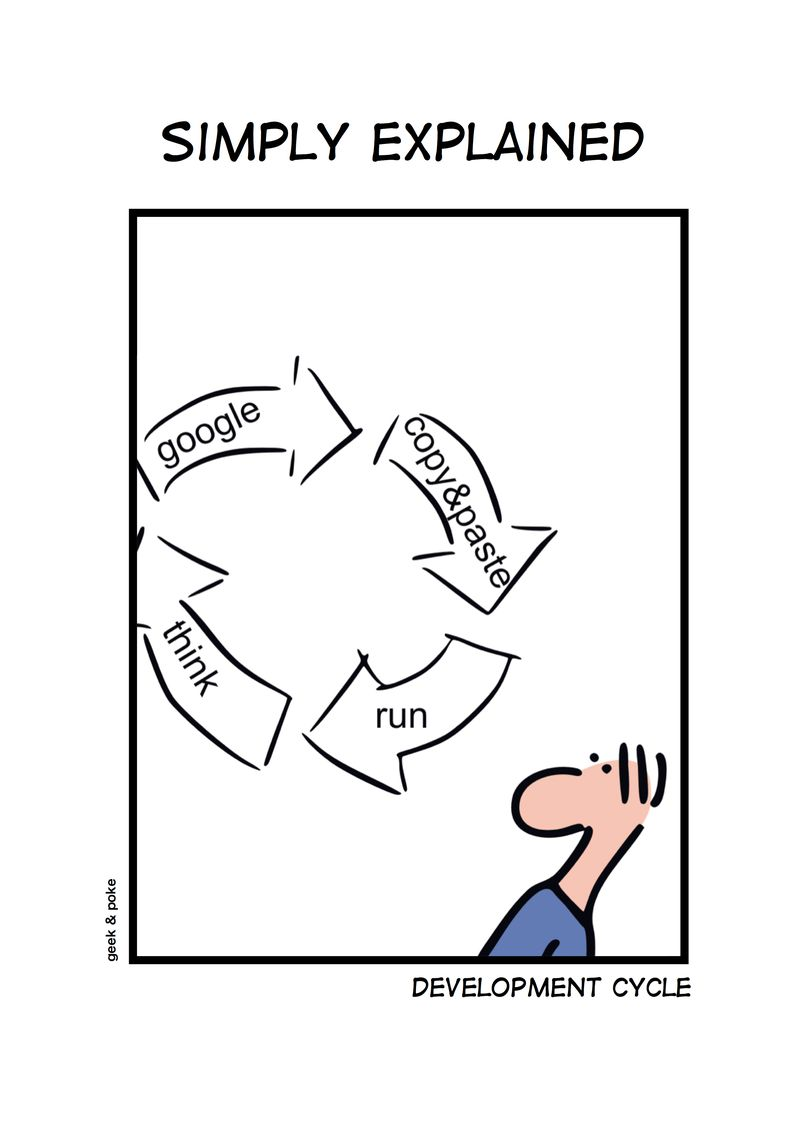
\includegraphics[scale=0.9]{./comics/geek_and_poke_development.jpg}
	\end{frame}

\end{document}